
\section{Methods}

\subsection{Data set}

The data used for the construction of the predictive models consists of 8708 samples
of different requests for funding from universities around the world, to finance research,
with the outcome being the success or failure of the request. The data set contains samples
from the years 2005 to 2008, with a total of 1882 predictors (independent variables). 
6633 samples from 2005 to 2007 and 1552 from 2008 were used for model training, and the 
remaining 518 samples from 2008 were used for testing the obtained model. Predictors can be 
separeted between continuous, such as the number of successes and failures passed by the 
``chief investigator'', and categorical ones, such as the monetary value of the grant, 
divided into 17 groups of increasing amounts, and the month of application.

\subsection{Preprocessing}

Initially, the first step is verifying the data skewness, in case there is a strong 
tendence to the left or to the right, an adequate transformation would be applied in order to 
remove the skewness. The next step is to scale and center the data around the mean. it is 
done so since different predictors can have different scales, and if they're not normalized,
models sensitive to the variance would be affected negatively, making it biased to those
predictors with the highest values. 

Then, what we should do is to verify which predictors have actual importance to the model 
construction, that is, which of them have a stronger say for the final prediction. We can 
study this by analysing their correlation. Those with a correlation larger than 0.99, with
zero variance or sparse, that is, that have lots of zero values as data, were removed.

Then, the final approach is to verify the linearity of the predictors together with the output. 
This step is essential, and the reason for this is, once we have analysed this aspect, we can
infer if using a linear model is the adequate way of resolving this problem. For example, 
if there are too much predictos with non-linear relationship with the final output, it makes no 
sense to insist in linear prediction models.

\subsection{Cross-Validation}

Cross-validation consists in a validation technique used to validate the model with the
test set, usually taking into account the model flexibility and the mean squared error (MSE).
Shortly, it divides the data set into $k$ distinct subsets of size as equal as 
possible. From these groups, one of them is put aside to be used as validation set,
while the model is trained based on the remaining $k-1$ subsets. Once the model is trained,
the first removed subset is used as validation as previously stated. Then, the removed 
subset is restored to the principal set, and the following subset is put aside to 
perform the same procedure until all of the $k$ subgroups are all used as validation set. 
This approach improves the model capability of generalization, once it is trained with 
all the data at dispose, it also makes the error estimation more robust.

This strategy generally serves to indicate which models have a better prediction capability
on the test set, since it enables the comparison between the error levels and the variance
generated.

it is important to state that if a $k$ is chosen such as it is too small, e.g, $k=2$ 
(two subgroups) or too large ($k=$sample size), we are going to have, respectively, a 
strongly biased model because we let a lot of data outside the training step, and a potential
overfitting issue due the high model complexity, ocurring the model to have a high variance.
Thus, to mitigate both of the effects, normally $k=5,10$ is employed, since they present
an acceptable level of bias and variance.

\subsection{Model validation performance}

One of the most used metrics to measure the performance a classification model is the
Receiver Operating Characteristic curve (ROC) and the Area Under the Curve (AUC). 
The ROC curve is traced in a graphic with the positive ratio in the y-axis and the negative
ratio in the x-axis, and each point of the curve is computed varying the classification
limiar. Decreasing this limiar makes the model classify more items as positive, increasing
the true positive and false positive. Increasing this limiar, causes the inverse
effect.

After calculating the ROC curve we can find the area under it. The area under the ROC curve
represents how well the model divides the two classes, as close the AUC value is from 1, 
better the model. However, this kind of analysis shouldn't be applied alone to validate
 a model's performance, since there is an information loss in the construction of the 
 graphic. Then, the dispersion table, which contains in its principal diagonal the number
 of true positives and true negatives, and in its secondary diagnoal the number of 
 false positives and false negatives, becomes an interesting analysis complement to the 
 ROC curve.

\subsection{Linear Methods}
\subsubsection{Logistic Regression (LR)}
It is statistical model used to determine the probability of an event. Therefora, its values 
are probabilities, which belong to the $(0,1)$ interval. 
The model is defined as:

\begin{equation}
   p(X) = \cfrac{e^{\beta_0 + \beta_1X}}{1+e^{\beta_0 + \beta_1X}} \hspace{0.15cm}, \hspace{0.35cm} 0\leq p(X) \leq 1 \label{eq1}
\end{equation}

This logistic model will aways produce a S-shaped curve, regardless of the value of $X$, 
getting a relatively precise prediction. After some mathematical astuces, it is possible 
to come up with the following equations that model the method.

\begin{equation}
    \cfrac{p(X)}{1-p(X)} = e^{\beta_0+\beta_1X} \label{eq2}
\end{equation}

\begin{equation}
    \log \left(\cfrac{p(X)}{1-p(X)}\right) = \beta_0+\beta_1X \label{eq3}
\end{equation}

The right term of Eq. \eqref{eq2} is called Odds, then the right term of Eq. \eqref{eq3} is 
called log-odds or logistic. The Odds ratio represents the effects of predictor X, on the
likelihood that an event will happen.

To adjust the model's parameters would be necessary to use
the Maximum-Likelihood technique to perform an estimation of them. However, it is also possible
to make use of the Least Squares for the adjust, as well as in the case of the 
coefficients in a linear regression.

\subsubsection{Linear Discriminant Analysis (LDA)}
Instead of directly estimating $P(Y|X)$, a model with the following characteristics will 
be developed:

\begin{itemize}
    \item Modeling the distribution of predictors of X separately in each class Y.
    \item Bayes' Theorem to estimate $P(Y = K|X = x)$.
    \item Normal distribution to describe each class.
\end{itemize}

Following from these informations, we initiate the model's development directly from the 
Bayes' Theorem:

\begin{equation}
    P(Y=k|X=x) = p_k(X) \label{eq4}
\end{equation}

\begin{equation}
    p_k(X) = \cfrac{P(X=x|Y=k)P(Y = k)}{P(X=x)} \label{eq5}
\end{equation}

\begin{equation}
    p_k(X) = \cfrac{\pi_k f_k(x)}{\sum^{K}_{l=1}\pi_lf_l(x)} \label{eq6}
\end{equation}

Where $f_k(x)$ represents the probability density function (pdf) of the r.a X of 
an observation belonging to class K. Thus, instead of directly computing $p_k(X)$ it is 
possible to simply estimate $\pi_k(X)$ and $f_k(X)$. Then, assuming that the number of 
predictors is unitary, we can make some affirmations about the form of $f_k(x)$ in order
to move on with the LDA method:

\begin{equation}
    f_k(x) = \cfrac{1}{\sqrt{2\pi\sigma^2_k}}e^{\cfrac{-(x-\mu_k)^2}{2\sigma^2_k}} \label{eq7}
\end{equation}

Besides, we assume $\sigma_1^2=...=\sigma_k^2$. Therefore, it is possible to write $p_k(X)$ 
as the following:

\begin{equation}
    p_k(X) = \cfrac{\pi_k \cfrac{1}{\sqrt{2\pi\sigma^2_k}}e^{\cfrac{-(x-\mu_k)^2}{2\sigma^2_k}}}{\sum^K_{l=1}\cfrac{1}{\sqrt{2\pi\sigma^2_l}}e^{\cfrac{-(x-\mu_l)^2}{2\sigma^2_l}}} \label{eq8}
\end{equation}

After some algebraic manipulations, it is possible to conclude that classifying one
observation to a given class is equivalent to classify one observation to a given class 
such that the the linear discriminant function $\sigma_k(x)$ is larger:

\begin{equation}
    \sigma_x = x\cfrac{\mu_x}{\sigma^2} - \cfrac{u_k^2}{2\sigma^2} + \log(\pi_k) \label{eq9}
\end{equation}

However, in practical situations, it is not always possible to know the parameter's values,
then LDA approximates the Bayes classifier by the following expressions:

\begin{equation}
    \hat{\mu_k} = \frac{1}{n_k} \sum^K_{i = k} x_i \label{eq10}
\end{equation}

\begin{equation}
    \hat{\sigma^2} = \frac{1}{n-K} \sum^K_{i = k} \sum^K_{i = k} (x_i-\hat{\mu_k})^2 \label{eq11}
\end{equation}

\begin{equation}
    \pi_k = \frac{n_k}{n}\label{eq12}
\end{equation}

\subsection{Non-Linear Methods}

\subsubsection{Support Vector Machine (SVM)}
\label{SVM}
In its simplest form, SVM separates points of two different classes using a single hyperplane with the Statistical Learning Technique~\cite{vapnik95, vapnik98}.
In the more complex versions, an hyperplane is built in $\mathbb{R}^n$, for a $n>2$, for 
the class split, the increase of $n$ leaves the problem with a non-linear solution. In general, it is used the expression in Eq. \eqref{eq19} to define the decision boundary, i.e, the hyperplane
for the separation of classes in $\mathbb{R}^2$.

\begin{equation}
    D(u)=\beta_0 + \sum_{j=1}^P \beta_j\mu_j = \beta_0+\sum_{i = 1}^ny_i\alpha_ix_i'u, \hspace{0.5cm} \alpha_i \geq 0 \label{eq19}
\end{equation}


\subsubsection{Decision Tree}
\label{Decision Tree}
This method is quite robust and it comes from a simple principle: divide the approach
into levels and attributes to build a cost function. To facilitate the visualization,
it is interesing to use a binary tree. In general, the approach is given by decision levels,
and for each level an attribute is chosen such that it better splits a data set 
according to the class.

\begin{figure}[htbp!]
    \centerline{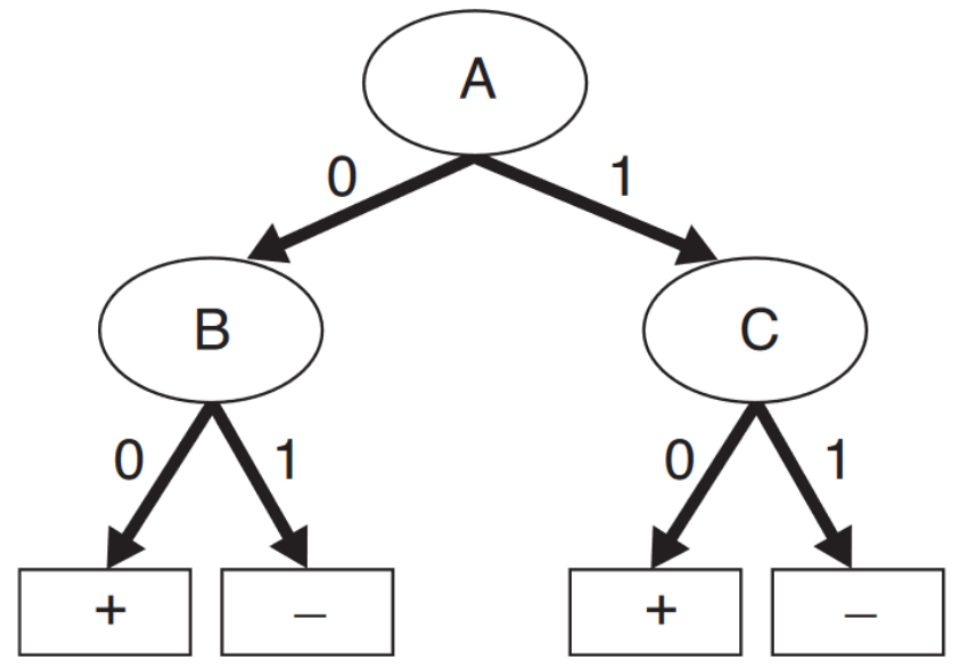
\includegraphics[width=0.3\textwidth]{fig1.png}}
    \caption{Example of a decision tree diagram. Figure from~\cite{Kumar2005}.}
    \label{fig:Tree}
  \end{figure}

For each new chosen attribute, new branches are created for the values present in the list
of all possible attributes values. The way this is implemented depends on the algorithm
used. In our work, we opted for the CART algorithm. The attributes choice in this model
is made based on the Gini Criterion, which deals with node impurity, defined in~\cite{breiman1984} as:

\begin{equation}
    \sum_{j \neq i} p(i|t)p(j|t) \label{eq20}
\end{equation}

In short, we can assume that the criterion associates an object randomly selected from a 
node to the class $i$ with probability $p(i|t)$. Meanwhile, $p(j|t)$ refers to the 
estimated error probability that the item belongs to class $j$, such that the $p(j|t)$
is the Gini Indice.

The Gini Criterion works with one class at a time, aiming to separate the more frequent 
class objects from the remaining objects in each test. 

The well detailed explanation it is really important, since one of the factors that may 
influence the precision and the time consumed to classify is the number of nodes present.

\begin{table*}[!htbp]
    \caption{Summarized results for each classification technique.}
    \begin{center}
    \begin{tabular}{|l|l|l|l|l|}
            \hline 
            Classifier & CV Accuracy ($\%$) & Train Time (s) & Test Time (s) ($\times 10^{-1}$)  \\
            \hline
            Logistic Regression & 83.78 & 12.93 & 0.175 \\
            \hline
            Linear Discriminant Analysis & 84.94 & 02.12 & 0.162 \\
            \hline
            SVM & 85.33 & 61.65 & 0.593 \\
            \hline
            Tree, 10 nodes & 83.20 & 00.84 &  0.131 \\
            \hline
            Tree, 100 nodes & 82.43 & 01.81 & 0.129 \\
            \hline
            KNN, $K = 1$ & 68.15 & 09.66 & 3.695 \\
            \hline
            KNN, $K = 50$ & 80.69 & 16.42 & 6.525 \\
            \hline
    \end{tabular}
  \label{tab:results}
  \end{center}
  \end{table*}

\subsubsection{K-Nearest Neighbors (KNN)} 
\label{KNN}
Generally in practice, informations about the conditional distribution of Y given X 
are not available. That being the case, the Bayes' classification method works only as 
a comparison tool to other more easily applicable practices. From this need of developing 
methods that don't rely on previous statements about the form of the boundary of decision,
the KNN routine takes place.

Shortly, KNN is a model such that its result is define by a ``voting'', where each ``vote'', 
is the amount of K samples closer of elements surrounding the analysed point which belongs
to a certain class. The class having the larger amount of points, or votes, wins. 

Something important to define in KNN methods is how the distances would be measured between
the samples, given that the classifiers are not in lenght units. Starting from this premise,
considering the vector $\textbf{x} = [p_{x_1}, ..., p_{x_n}]$, and $\textbf{n} = [p_{n_1}, ..., p_{n_n}]$, 
where $\textbf{x}$ the vector that represents the sample to be classified and $\textbf{v}$
is the neighbor vector to be computed the distance. Therefore, the most traditional way 
of computing the distance, is using the Euclidian Distance:

\begin{equation}
    d = \sqrt{\langle (x-v), (x-v)\rangle} \label{eq16}
\end{equation}

There is various methods to compute the distance between the sample. In the training phase, the best results were obtained by using the Spearman Distance computation
method, since it present more robustness against outliers. On the other hand, there is a loss of information when data are converted~\cite{Kumar2014}. It is represented by $\overline{(\cdot)}$,
given as: 

\begin{equation}
    d = 1 - \cfrac{\langle (x-\overline{x}), (v - \overline{v})\rangle}{\langle \sqrt{\langle (x-\overline{x}), (v - \overline{v})\rangle}, \sqrt{\langle (x-\overline{x}), (v - \overline{v})\rangle}\rangle}
\end{equation}

This distance was used in a test with 50 neighbors, together with the use of weights that
considered the inverse of the square distance, and in order to not harm its performance, 
the data weren't standardized, being the second more well succeeded than
the previous and also than the pure distance. However, by means of reference, the proposed 
experiments are computed without weights and with Euclidian Distance.

Since KNN does not classify the samples by probabilities, one way of making it possible is to 
make the probabilities related to votes of each sample. This is done by the following 
equation. which defines the conditional probabilities, with $K \in \mathbb{Z}^{+}$ referent 
to the neighbors and an observation $x_0$ in a set $N_0$ and the function $I(\cdot)$
returns 1 if the sample $y_i \neq j$ and 0 otherwise.

\begin{equation}
    P(Y = j|X = x_0) = \frac{1}{K} \sum_{i \in N_0} I(y_i = j) 
\end{equation}

Finally, to conclude the KNN algorithm the Bayes' Rule must be applied to classify the 
observations $x_0$ into the class with the highest probability of occurence. It is 
interesing to notice that for $K$ close to 1, the decision boundary is extremely 
flexible, corresponding to a classifier with low bias and high variance. For large K, the situation is the inverse.